% Ich teile hier einfach mal meine Erfahrung der letzten Stunde trouble shooting.
% Latex = alles gut
% Bibtex = Denk einfach nich daran Umlaute zu benutzen. Nicht in der Bibliography, und auch nicht in Dateinamen
% Im eigentlichen Text gehts. Sachen wie Carrá sind aus irgendeinem Grund wiederum erlaubt, auch in der Bibliography
% Fix: {\"o} statt ö etc. (inkl. eckigen Klammern)

\chapter{Einführung}

Dieses Dokument, welches die Ausarbeitung zum Thema \glqq DevOps\grqq\ im Modul Software-Entwicklungsprozesse darstellt, stellt am Anfang die herkömmliche Unternehmenskultur und ihre Vor- sowie Nachteile dar. Im Zuge dieser Vorstellung wird dem Leser klar, warum diese Unternehmenskultur auf mittelfristige Sicht nicht funktionieren kann und zu Problemen führt. Als eine mögliche Lösung für diese Probleme wird dann das Konzept der \ac{DevOps}-Philosophie vorgestellt. Hierzu wird zuerst kurz der Ursprung des \ac{DevOps} aufgezeigt, danach werden die Leitsätze und wichtigsten Prinzipien erklärt sowie auch einige Kritikpunkte an \ac{DevOps} beschrieben und abgehandelt.\\
Im nächsten Schritt wird ein grundsätzliches Modell vorgestellt, das Helfen kann, den Übergang von einer herkömmlichen Unternehmenskultur hin zu \ac{DevOps} zu bewerkstelligen. Außerdem werden auch einige Schritte genannt, die kontinuierlich vollzogen werden müssen, um \ac{DevOps} effizient gestalten zu können.\\
Am Ende der Ausarbeitung wird ein kleines Bild der realen Welt in der Industrie gezeichnet, z. B. wie weit \ac{DevOps} verbreitet ist bzw. warum es nicht genutzt wird usw.

\section{Herkömmliche Unternehmenskultur}

\begin{figure}[hb]
\centering
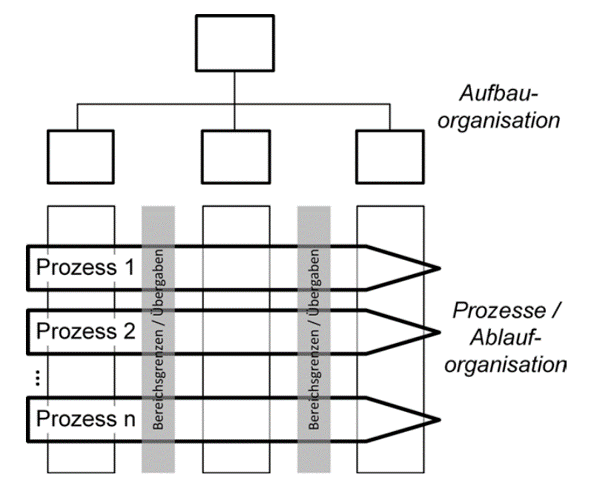
\includegraphics[width=0.7\textwidth]{Graphics/silodenken}
\caption{Silodenken \cite{halstenberg:2020}}
\label{fig:silo}
\end{figure}

Eine Darstellung einer einfachen, herkömmlichen Unternehmenskultur ist in \autoref{fig:silo} zu sehen. Diese Art von Unternehmenskultur wird auch \glqq Silodenke\grqq\ genannt, benannt nach den in der Abbildung zu erkennenden Silos, welche durch die vertikalen Balken dargestellt sind. Veranschaulicht werden damit z. B. die verschiedenen Abteilungen oder Teams innerhalb der Unternehmensstruktur. Obwohl es mehrere Team-übergreifende Prozesse gibt (dargestellt durch die horizontalen Pfeile, die mehrere der Silos verbinden), bei denen die einzelnen Teams miteinander arbeiten müssen, ist ein extremer Zusammenhalt innerhalb dieser Teams und vor allem eine rivalisierende Haltung gegenüber anderen Teams zu erkennen. Es wird mehr gegeneinander in Teams gearbeitet als miteinander für den Prozess. In dieser Unternehmenskultur wird somit in sogenannten Silos gedacht, den voneinander abgekapselten einzelnen Teams. Diese Art zu denken ist durch ein starkes Gefühl der Gruppenzugehörigkeit in der Natur des Menschen insgesamt sehr tief verankert und ist damit eine sehr intuitive Art zu  denken. Einen gewissen sofortigen Vorteil für die einzelne Person bzw. die Teams hat diese Art der Denke natürlich auch, meistens hilft es im ersten Moment dabei, Arbeit abzuwälzen und Prozesse sehr selbstorientiert zu absolvieren. Mittelfristig führt die Silodenke aber zu großen Problemen innerhalb des Unternehmens und der Silo-übergreifenden Prozesse.

\section{Wall of Confusion}

Wenn jeder so denkt, wie im vorherigen Abschnitt mit der Silodenke beschrieben, so führt dies dazu, dass niemand in Kommunikation mit anderen Teams tritt, um den Prozess insgesamt effizienter zu gestalten. Jeder führt seinen Teilprozess so aus, dass es am wenigsten Arbeit für ihn generiert und wirft das Endprodukt sozusagen \glqq über den Zaun\grqq. Mit Zaun sind die in \autoref{fig:silo} zu sehenden grauen, vertikalen Balken gemeint, die zwischen den Silos stehen und die übergreifenden Prozesse unterbrechen, welche auch \glqq Wall of Confusion\grqq\ genannt werden. Es auf den ersten Blick so aus, dass man damit sich und seinem Team weniger Arbeit macht, weil unser Endprodukt nicht auf das folgende Team ausgelegt ist. Das Problem dabei ist jedoch, wenn jedes Team so denkt, bekommt auch das eigene Team als zu verarbeitendes Produkt etwas, das vom vorherigen Team nur über den Zaun geworfen wurde. Somit muss auch das eigene Team einen Mehraufwand aufbringen, um den benötigten Teilprozess abarbeiten zu können.

\begin{figure}[h]
\centering
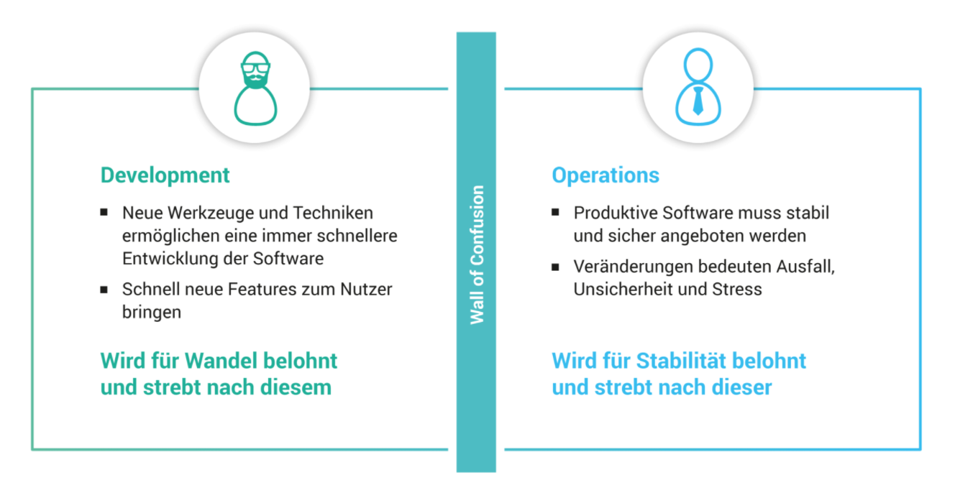
\includegraphics[width=0.8\textwidth]{Graphics/wall_of_confusion}
\caption{Wall Of Confusion \cite{novatec:2021}}
\label{fig:wall}
\end{figure}

In \autoref{fig:wall} ist eine solche Wall of Confusion beispielhaft für die Abteilungen des Developments und der Operations aufgezeigt und spezifiziert. Klar zu sehen ist, dass die beiden Abteilungen absolut gegensätzliche Ziele bei der Entwicklung und Verbesserung des Endprodukts haben. Auf der einen Seite das Development, welches gerne experimentiert, neue Features und Tools in kurzen Zyklen schnell implementieren und zum Kunden bringen will. Auf der anderen Seite die Operations, die wollen, dass das Endprodukt stabil und sicher beim Kunden ankommt und dort keine Probleme verursacht, also lange Zyklen, viel Testen, wenig Risiko.\\
Das Ziel ist es nun, diese Wall of Confusion mit ihren gegensätzlichen Ansichten auf beiden Seiten irgendwie zu überwinden und die Zusammenarbeit der beiden Abteilungen effizienter, weniger spannungsgeladen und angenehmer zu gestalten. Hierfür wird nun in der folgenden Ausarbeitung die Philosophie des \ac{DevOps} vorgestellt. 
